

\tikzset{every picture/.style={line width=0.75pt}} %set default line width to 0.75pt        

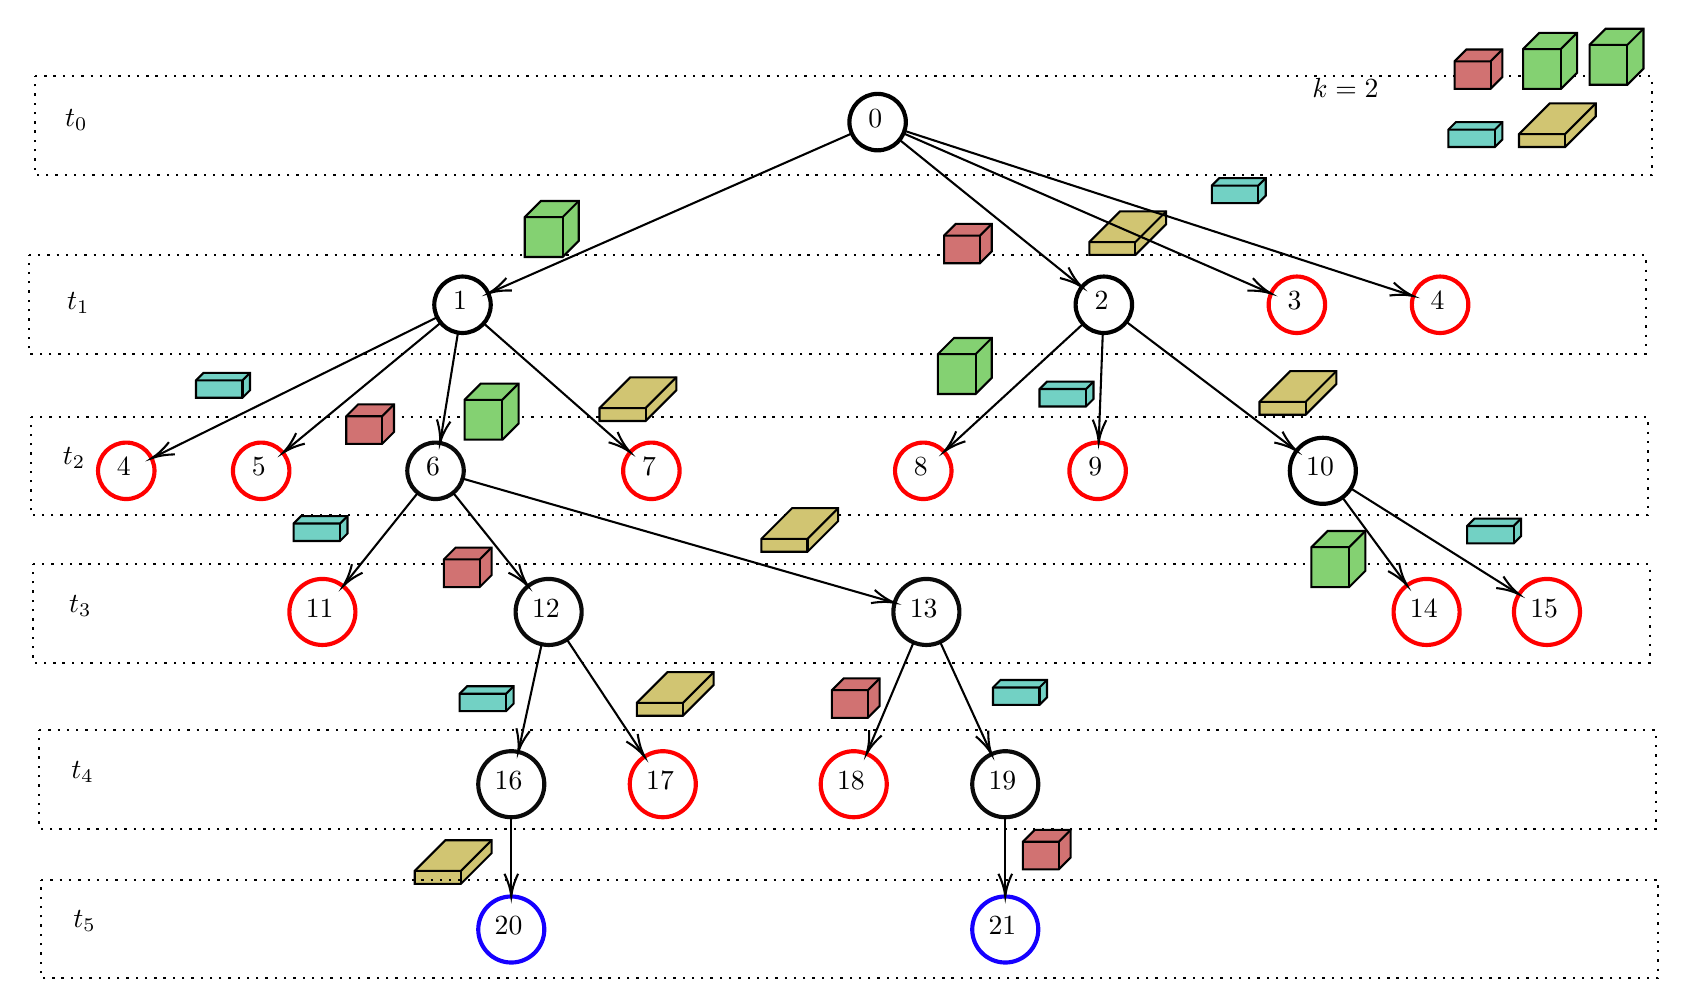
\begin{tikzpicture}[x=0.75pt,y=0.75pt,yscale=-1,xscale=1]
%uncomment if require: \path (0,685); %set diagram left start at 0, and has height of 685

%Shape: Rectangle [id:dp7518152982306099] 
\draw  [dash pattern={on 0.84pt off 2.51pt}] (33,41) -- (812,41) -- (812,88.5) -- (33,88.5) -- cycle ;
%Shape: Rectangle [id:dp3153529928931591] 
\draw  [dash pattern={on 0.84pt off 2.51pt}] (32,276) -- (811,276) -- (811,323.5) -- (32,323.5) -- cycle ;
%Shape: Rectangle [id:dp30504334488182117] 
\draw  [dash pattern={on 0.84pt off 2.51pt}] (30,127) -- (809,127) -- (809,174.5) -- (30,174.5) -- cycle ;
%Shape: Rectangle [id:dp8769552866501534] 
\draw  [dash pattern={on 0.84pt off 2.51pt}] (31,205) -- (810,205) -- (810,252.5) -- (31,252.5) -- cycle ;
%Shape: Cube [id:dp8832506159680754] 
\draw  [fill={rgb, 255:red, 209; green, 114; blue, 114 }  ,fill opacity=1 ] (717,33.7) -- (722.7,28) -- (740,28) -- (740,41.3) -- (734.3,47) -- (717,47) -- cycle ; \draw   (740,28) -- (734.3,33.7) -- (717,33.7) ; \draw   (734.3,33.7) -- (734.3,47) ;
%Shape: Cube [id:dp17567715950752727] 
\draw  [fill={rgb, 255:red, 132; green, 209; blue, 114 }  ,fill opacity=1 ] (750,27.8) -- (757.8,20) -- (776,20) -- (776,39.2) -- (768.2,47) -- (750,47) -- cycle ; \draw   (776,20) -- (768.2,27.8) -- (750,27.8) ; \draw   (768.2,27.8) -- (768.2,47) ;
%Shape: Cube [id:dp10020806396004756] 
\draw  [fill={rgb, 255:red, 114; green, 209; blue, 196 }  ,fill opacity=1 ] (714,66.6) -- (717.6,63) -- (740,63) -- (740,71.4) -- (736.4,75) -- (714,75) -- cycle ; \draw   (740,63) -- (736.4,66.6) -- (714,66.6) ; \draw   (736.4,66.6) -- (736.4,75) ;
%Shape: Cube [id:dp6815153362050183] 
\draw  [fill={rgb, 255:red, 209; green, 197; blue, 114 }  ,fill opacity=1 ] (748,68.78) -- (762.78,54) -- (785,54) -- (785,60.22) -- (770.22,75) -- (748,75) -- cycle ; \draw   (785,54) -- (770.22,68.78) -- (748,68.78) ; \draw   (770.22,68.78) -- (770.22,75) ;
%Shape: Cube [id:dp9055300095738211] 
\draw  [fill={rgb, 255:red, 132; green, 209; blue, 114 }  ,fill opacity=1 ] (269,108.8) -- (276.8,101) -- (295,101) -- (295,120.2) -- (287.2,128) -- (269,128) -- cycle ; \draw   (295,101) -- (287.2,108.8) -- (269,108.8) ; \draw   (287.2,108.8) -- (287.2,128) ;
%Shape: Cube [id:dp8748590504863185] 
\draw  [fill={rgb, 255:red, 209; green, 114; blue, 114 }  ,fill opacity=1 ] (471,117.7) -- (476.7,112) -- (494,112) -- (494,125.3) -- (488.3,131) -- (471,131) -- cycle ; \draw   (494,112) -- (488.3,117.7) -- (471,117.7) ; \draw   (488.3,117.7) -- (488.3,131) ;
%Shape: Cube [id:dp5094935254839879] 
\draw  [fill={rgb, 255:red, 209; green, 197; blue, 114 }  ,fill opacity=1 ] (541,120.78) -- (555.78,106) -- (578,106) -- (578,112.22) -- (563.22,127) -- (541,127) -- cycle ; \draw   (578,106) -- (563.22,120.78) -- (541,120.78) ; \draw   (563.22,120.78) -- (563.22,127) ;
%Shape: Cube [id:dp2584826139567201] 
\draw  [fill={rgb, 255:red, 114; green, 209; blue, 196 }  ,fill opacity=1 ] (600,93.6) -- (603.6,90) -- (626,90) -- (626,98.4) -- (622.4,102) -- (600,102) -- cycle ; \draw   (626,90) -- (622.4,93.6) -- (600,93.6) ; \draw   (622.4,93.6) -- (622.4,102) ;
%Shape: Cube [id:dp35162087734757685] 
\draw  [fill={rgb, 255:red, 132; green, 209; blue, 114 }  ,fill opacity=1 ] (468,174.8) -- (475.8,167) -- (494,167) -- (494,186.2) -- (486.2,194) -- (468,194) -- cycle ; \draw   (494,167) -- (486.2,174.8) -- (468,174.8) ; \draw   (486.2,174.8) -- (486.2,194) ;
%Shape: Cube [id:dp910995187687212] 
\draw  [fill={rgb, 255:red, 114; green, 209; blue, 196 }  ,fill opacity=1 ] (517,191.6) -- (520.6,188) -- (543,188) -- (543,196.4) -- (539.4,200) -- (517,200) -- cycle ; \draw   (543,188) -- (539.4,191.6) -- (517,191.6) ; \draw   (539.4,191.6) -- (539.4,200) ;
%Shape: Cube [id:dp736751641806709] 
\draw  [fill={rgb, 255:red, 209; green, 197; blue, 114 }  ,fill opacity=1 ] (623,197.78) -- (637.78,183) -- (660,183) -- (660,189.22) -- (645.22,204) -- (623,204) -- cycle ; \draw   (660,183) -- (645.22,197.78) -- (623,197.78) ; \draw   (645.22,197.78) -- (645.22,204) ;
%Shape: Cube [id:dp5718821249322832] 
\draw  [fill={rgb, 255:red, 114; green, 209; blue, 196 }  ,fill opacity=1 ] (110.6,187.4) -- (114.2,183.8) -- (136.6,183.8) -- (136.6,192.2) -- (133,195.8) -- (110.6,195.8) -- cycle ; \draw   (136.6,183.8) -- (133,187.4) -- (110.6,187.4) ; \draw   (133,187.4) -- (133,195.8) ;
%Shape: Cube [id:dp12731759956147481] 
\draw  [fill={rgb, 255:red, 209; green, 197; blue, 114 }  ,fill opacity=1 ] (305,200.78) -- (319.78,186) -- (342,186) -- (342,192.22) -- (327.22,207) -- (305,207) -- cycle ; \draw   (342,186) -- (327.22,200.78) -- (305,200.78) ; \draw   (327.22,200.78) -- (327.22,207) ;
%Shape: Cube [id:dp49728154886725173] 
\draw  [fill={rgb, 255:red, 209; green, 114; blue, 114 }  ,fill opacity=1 ] (183,204.7) -- (188.7,199) -- (206,199) -- (206,212.3) -- (200.3,218) -- (183,218) -- cycle ; \draw   (206,199) -- (200.3,204.7) -- (183,204.7) ; \draw   (200.3,204.7) -- (200.3,218) ;
%Shape: Cube [id:dp42948149944958625] 
\draw  [fill={rgb, 255:red, 132; green, 209; blue, 114 }  ,fill opacity=1 ] (782,25.8) -- (789.8,18) -- (808,18) -- (808,37.2) -- (800.2,45) -- (782,45) -- cycle ; \draw   (808,18) -- (800.2,25.8) -- (782,25.8) ; \draw   (800.2,25.8) -- (800.2,45) ;
%Shape: Cube [id:dp3074913486852153] 
\draw  [fill={rgb, 255:red, 132; green, 209; blue, 114 }  ,fill opacity=1 ] (240,196.8) -- (247.8,189) -- (266,189) -- (266,208.2) -- (258.2,216) -- (240,216) -- cycle ; \draw   (266,189) -- (258.2,196.8) -- (240,196.8) ; \draw   (258.2,196.8) -- (258.2,216) ;
%Shape: Cube [id:dp8270523351282212] 
\draw  [fill={rgb, 255:red, 114; green, 209; blue, 196 }  ,fill opacity=1 ] (157.6,256.4) -- (161.2,252.8) -- (183.6,252.8) -- (183.6,261.2) -- (180,264.8) -- (157.6,264.8) -- cycle ; \draw   (183.6,252.8) -- (180,256.4) -- (157.6,256.4) ; \draw   (180,256.4) -- (180,264.8) ;
%Shape: Cube [id:dp16888670014841067] 
\draw  [fill={rgb, 255:red, 209; green, 197; blue, 114 }  ,fill opacity=1 ] (383,263.78) -- (397.78,249) -- (420,249) -- (420,255.22) -- (405.22,270) -- (383,270) -- cycle ; \draw   (420,249) -- (405.22,263.78) -- (383,263.78) ; \draw   (405.22,263.78) -- (405.22,270) ;
%Shape: Cube [id:dp1783428693721696] 
\draw  [fill={rgb, 255:red, 209; green, 114; blue, 114 }  ,fill opacity=1 ] (230,273.7) -- (235.7,268) -- (253,268) -- (253,281.3) -- (247.3,287) -- (230,287) -- cycle ; \draw   (253,268) -- (247.3,273.7) -- (230,273.7) ; \draw   (247.3,273.7) -- (247.3,287) ;
%Shape: Cube [id:dp15995921210500508] 
\draw  [fill={rgb, 255:red, 132; green, 209; blue, 114 }  ,fill opacity=1 ] (648,267.8) -- (655.8,260) -- (674,260) -- (674,279.2) -- (666.2,287) -- (648,287) -- cycle ; \draw   (674,260) -- (666.2,267.8) -- (648,267.8) ; \draw   (666.2,267.8) -- (666.2,287) ;
%Shape: Cube [id:dp19462080035867757] 
\draw  [fill={rgb, 255:red, 114; green, 209; blue, 196 }  ,fill opacity=1 ] (723,257.6) -- (726.6,254) -- (749,254) -- (749,262.4) -- (745.4,266) -- (723,266) -- cycle ; \draw   (749,254) -- (745.4,257.6) -- (723,257.6) ; \draw   (745.4,257.6) -- (745.4,266) ;
%Shape: Cube [id:dp3532873019701165] 
\draw  [fill={rgb, 255:red, 209; green, 197; blue, 114 }  ,fill opacity=1 ] (323,342.78) -- (337.78,328) -- (360,328) -- (360,334.22) -- (345.22,349) -- (323,349) -- cycle ; \draw   (360,328) -- (345.22,342.78) -- (323,342.78) ; \draw   (345.22,342.78) -- (345.22,349) ;
%Shape: Cube [id:dp5913596168061985] 
\draw  [fill={rgb, 255:red, 114; green, 209; blue, 196 }  ,fill opacity=1 ] (237.6,338.4) -- (241.2,334.8) -- (263.6,334.8) -- (263.6,343.2) -- (260,346.8) -- (237.6,346.8) -- cycle ; \draw   (263.6,334.8) -- (260,338.4) -- (237.6,338.4) ; \draw   (260,338.4) -- (260,346.8) ;
%Shape: Cube [id:dp8066047594137742] 
\draw  [fill={rgb, 255:red, 209; green, 114; blue, 114 }  ,fill opacity=1 ] (417,336.7) -- (422.7,331) -- (440,331) -- (440,344.3) -- (434.3,350) -- (417,350) -- cycle ; \draw   (440,331) -- (434.3,336.7) -- (417,336.7) ; \draw   (434.3,336.7) -- (434.3,350) ;
%Shape: Cube [id:dp030204008242722513] 
\draw  [fill={rgb, 255:red, 114; green, 209; blue, 196 }  ,fill opacity=1 ] (494.6,335.4) -- (498.2,331.8) -- (520.6,331.8) -- (520.6,340.2) -- (517,343.8) -- (494.6,343.8) -- cycle ; \draw   (520.6,331.8) -- (517,335.4) -- (494.6,335.4) ; \draw   (517,335.4) -- (517,343.8) ;
%Shape: Cube [id:dp8580618024500212] 
\draw  [fill={rgb, 255:red, 209; green, 114; blue, 114 }  ,fill opacity=1 ] (509,409.7) -- (514.7,404) -- (532,404) -- (532,417.3) -- (526.3,423) -- (509,423) -- cycle ; \draw   (532,404) -- (526.3,409.7) -- (509,409.7) ; \draw   (526.3,409.7) -- (526.3,423) ;
%Shape: Cube [id:dp5613856379149467] 
\draw  [fill={rgb, 255:red, 209; green, 197; blue, 114 }  ,fill opacity=1 ] (216,423.78) -- (230.78,409) -- (253,409) -- (253,415.22) -- (238.22,430) -- (216,430) -- cycle ; \draw   (253,409) -- (238.22,423.78) -- (216,423.78) ; \draw   (238.22,423.78) -- (238.22,430) ;
%Shape: Rectangle [id:dp8504421355642154] 
\draw  [dash pattern={on 0.84pt off 2.51pt}] (35,356) -- (814,356) -- (814,403.5) -- (35,403.5) -- cycle ;
%Shape: Rectangle [id:dp46457948980853214] 
\draw  [dash pattern={on 0.84pt off 2.51pt}] (36,428) -- (815,428) -- (815,475.5) -- (36,475.5) -- cycle ;

% Text Node
\draw  [line width=1.5]   (439, 63) circle [x radius= 13.6, y radius= 13.6]   ;
\draw (433,55.4) node [anchor=north west][inner sep=0.75pt]    {$0$};
% Text Node
\draw  [line width=1.5]   (239, 151) circle [x radius= 13.6, y radius= 13.6]   ;
\draw (233,143.4) node [anchor=north west][inner sep=0.75pt]    {$1$};
% Text Node
\draw  [line width=1.5]   (548, 151) circle [x radius= 13.6, y radius= 13.6]   ;
\draw (542,143.4) node [anchor=north west][inner sep=0.75pt]    {$2$};
% Text Node
\draw  [color={rgb, 255:red, 255; green, 0; blue, 0 }  ,draw opacity=1 ][line width=1.5]   (641, 151) circle [x radius= 13.6, y radius= 13.6]   ;
\draw (635,143.4) node [anchor=north west][inner sep=0.75pt]    {$3$};
% Text Node
\draw  [color={rgb, 255:red, 255; green, 0; blue, 0 }  ,draw opacity=1 ][line width=1.5]   (710, 151) circle [x radius= 13.6, y radius= 13.6]   ;
\draw (704,143.4) node [anchor=north west][inner sep=0.75pt]    {$4$};
% Text Node
\draw  [color={rgb, 255:red, 255; green, 0; blue, 0 }  ,draw opacity=1 ][line width=1.5]   (142, 231) circle [x radius= 13.6, y radius= 13.6]   ;
\draw (136,223.4) node [anchor=north west][inner sep=0.75pt]    {$5$};
% Text Node
\draw  [color={rgb, 255:red, 10; green, 10; blue, 10 }  ,draw opacity=1 ][line width=1.5]   (226, 231) circle [x radius= 13.6, y radius= 13.6]   ;
\draw (220,223.4) node [anchor=north west][inner sep=0.75pt]    {$6$};
% Text Node
\draw  [color={rgb, 255:red, 255; green, 0; blue, 0 }  ,draw opacity=1 ][line width=1.5]   (330, 231) circle [x radius= 13.6, y radius= 13.6]   ;
\draw (324,223.4) node [anchor=north west][inner sep=0.75pt]    {$7$};
% Text Node
\draw  [color={rgb, 255:red, 255; green, 0; blue, 0 }  ,draw opacity=1 ][line width=1.5]   (461, 231) circle [x radius= 13.6, y radius= 13.6]   ;
\draw (455,223.4) node [anchor=north west][inner sep=0.75pt]    {$8$};
% Text Node
\draw  [color={rgb, 255:red, 255; green, 0; blue, 0 }  ,draw opacity=1 ][line width=1.5]   (545, 231) circle [x radius= 13.6, y radius= 13.6]   ;
\draw (539,223.4) node [anchor=north west][inner sep=0.75pt]    {$9$};
% Text Node
\draw  [line width=1.5]   (653.5, 231) circle [x radius= 15.91, y radius= 15.91]   ;
\draw (644,223.4) node [anchor=north west][inner sep=0.75pt]    {$10$};
% Text Node
\draw  [color={rgb, 255:red, 255; green, 0; blue, 0 }  ,draw opacity=1 ][line width=1.5]   (77, 231) circle [x radius= 13.6, y radius= 13.6]   ;
\draw (71,223.4) node [anchor=north west][inner sep=0.75pt]    {$4$};
% Text Node
\draw  [color={rgb, 255:red, 255; green, 0; blue, 0 }  ,draw opacity=1 ][line width=1.5]   (171.5, 299) circle [x radius= 15.91, y radius= 15.91]   ;
\draw (162,291.4) node [anchor=north west][inner sep=0.75pt]    {$11$};
% Text Node
\draw  [color={rgb, 255:red, 10; green, 10; blue, 10 }  ,draw opacity=1 ][line width=1.5]   (280.5, 299) circle [x radius= 15.91, y radius= 15.91]   ;
\draw (271,291.4) node [anchor=north west][inner sep=0.75pt]    {$12$};
% Text Node
\draw  [color={rgb, 255:red, 10; green, 10; blue, 10 }  ,draw opacity=1 ][line width=1.5]   (462.5, 299) circle [x radius= 15.91, y radius= 15.91]   ;
\draw (453,291.4) node [anchor=north west][inner sep=0.75pt]    {$13$};
% Text Node
\draw  [color={rgb, 255:red, 255; green, 0; blue, 0 }  ,draw opacity=1 ][line width=1.5]   (703.5, 299) circle [x radius= 15.91, y radius= 15.91]   ;
\draw (694,291.4) node [anchor=north west][inner sep=0.75pt]    {$14$};
% Text Node
\draw  [color={rgb, 255:red, 255; green, 0; blue, 0 }  ,draw opacity=1 ][line width=1.5]   (761.5, 299) circle [x radius= 15.91, y radius= 15.91]   ;
\draw (752,291.4) node [anchor=north west][inner sep=0.75pt]    {$15$};
% Text Node
\draw (647,40.4) node [anchor=north west][inner sep=0.75pt]    {$k=2$};
% Text Node
\draw (46,55.4) node [anchor=north west][inner sep=0.75pt]    {$t_{0}$};
% Text Node
\draw (47,143.4) node [anchor=north west][inner sep=0.75pt]    {$t_{1}$};
% Text Node
\draw (45,218.4) node [anchor=north west][inner sep=0.75pt]    {$t_{2}$};
% Text Node
\draw (48,289.4) node [anchor=north west][inner sep=0.75pt]    {$t_{3}$};
% Text Node
\draw  [color={rgb, 255:red, 10; green, 10; blue, 10 }  ,draw opacity=1 ][line width=1.5]   (262.5, 382) circle [x radius= 15.91, y radius= 15.91]   ;
\draw (253,374.4) node [anchor=north west][inner sep=0.75pt]    {$16$};
% Text Node
\draw  [color={rgb, 255:red, 255; green, 0; blue, 0 }  ,draw opacity=1 ][line width=1.5]   (335.5, 382) circle [x radius= 15.91, y radius= 15.91]   ;
\draw (326,374.4) node [anchor=north west][inner sep=0.75pt]    {$17$};
% Text Node
\draw  [color={rgb, 255:red, 255; green, 0; blue, 0 }  ,draw opacity=1 ][line width=1.5]   (427.5, 382) circle [x radius= 15.91, y radius= 15.91]   ;
\draw (418,374.4) node [anchor=north west][inner sep=0.75pt]    {$18$};
% Text Node
\draw  [color={rgb, 255:red, 10; green, 10; blue, 10 }  ,draw opacity=1 ][line width=1.5]   (500.5, 382) circle [x radius= 15.91, y radius= 15.91]   ;
\draw (491,374.4) node [anchor=north west][inner sep=0.75pt]    {$19$};
% Text Node
\draw  [color={rgb, 255:red, 21; green, 0; blue, 255 }  ,draw opacity=1 ][line width=1.5]   (262.5, 452) circle [x radius= 15.91, y radius= 15.91]   ;
\draw (253,444.4) node [anchor=north west][inner sep=0.75pt]    {$20$};
% Text Node
\draw  [color={rgb, 255:red, 21; green, 0; blue, 255 }  ,draw opacity=1 ][line width=1.5]   (500.5, 452) circle [x radius= 15.91, y radius= 15.91]   ;
\draw (491,444.4) node [anchor=north west][inner sep=0.75pt]    {$21$};
% Text Node
\draw (49,369.4) node [anchor=north west][inner sep=0.75pt]    {$t_{4}$};
% Text Node
\draw (50,441.4) node [anchor=north west][inner sep=0.75pt]    {$t_{5}$};
% Connection
\draw    (426.55,68.48) -- (253.28,144.72) ;
\draw [shift={(251.45,145.52)}, rotate = 336.25] [color={rgb, 255:red, 0; green, 0; blue, 0 }  ][line width=0.75]    (10.93,-3.29) .. controls (6.95,-1.4) and (3.31,-0.3) .. (0,0) .. controls (3.31,0.3) and (6.95,1.4) .. (10.93,3.29)   ;
% Connection
\draw    (449.58,71.54) -- (535.86,141.2) ;
\draw [shift={(537.42,142.46)}, rotate = 218.92] [color={rgb, 255:red, 0; green, 0; blue, 0 }  ][line width=0.75]    (10.93,-3.29) .. controls (6.95,-1.4) and (3.31,-0.3) .. (0,0) .. controls (3.31,0.3) and (6.95,1.4) .. (10.93,3.29)   ;
% Connection
\draw    (451.47,68.43) -- (626.69,144.77) ;
\draw [shift={(628.53,145.57)}, rotate = 203.54] [color={rgb, 255:red, 0; green, 0; blue, 0 }  ][line width=0.75]    (10.93,-3.29) .. controls (6.95,-1.4) and (3.31,-0.3) .. (0,0) .. controls (3.31,0.3) and (6.95,1.4) .. (10.93,3.29)   ;
% Connection
\draw    (451.94,67.2) -- (695.16,146.18) ;
\draw [shift={(697.06,146.8)}, rotate = 197.99] [color={rgb, 255:red, 0; green, 0; blue, 0 }  ][line width=0.75]    (10.93,-3.29) .. controls (6.95,-1.4) and (3.31,-0.3) .. (0,0) .. controls (3.31,0.3) and (6.95,1.4) .. (10.93,3.29)   ;
% Connection
\draw    (228.51,159.65) -- (154.04,221.07) ;
\draw [shift={(152.49,222.35)}, rotate = 320.49] [color={rgb, 255:red, 0; green, 0; blue, 0 }  ][line width=0.75]    (10.93,-3.29) .. controls (6.95,-1.4) and (3.31,-0.3) .. (0,0) .. controls (3.31,0.3) and (6.95,1.4) .. (10.93,3.29)   ;
% Connection
\draw    (236.82,164.43) -- (228.5,215.6) ;
\draw [shift={(228.18,217.57)}, rotate = 279.23] [color={rgb, 255:red, 0; green, 0; blue, 0 }  ][line width=0.75]    (10.93,-3.29) .. controls (6.95,-1.4) and (3.31,-0.3) .. (0,0) .. controls (3.31,0.3) and (6.95,1.4) .. (10.93,3.29)   ;
% Connection
\draw    (249.22,159.98) -- (318.28,220.7) ;
\draw [shift={(319.78,222.02)}, rotate = 221.32] [color={rgb, 255:red, 0; green, 0; blue, 0 }  ][line width=0.75]    (10.93,-3.29) .. controls (6.95,-1.4) and (3.31,-0.3) .. (0,0) .. controls (3.31,0.3) and (6.95,1.4) .. (10.93,3.29)   ;
% Connection
\draw    (537.99,160.21) -- (472.48,220.44) ;
\draw [shift={(471.01,221.79)}, rotate = 317.4] [color={rgb, 255:red, 0; green, 0; blue, 0 }  ][line width=0.75]    (10.93,-3.29) .. controls (6.95,-1.4) and (3.31,-0.3) .. (0,0) .. controls (3.31,0.3) and (6.95,1.4) .. (10.93,3.29)   ;
% Connection
\draw    (547.49,164.59) -- (545.58,215.41) ;
\draw [shift={(545.51,217.41)}, rotate = 272.15] [color={rgb, 255:red, 0; green, 0; blue, 0 }  ][line width=0.75]    (10.93,-3.29) .. controls (6.95,-1.4) and (3.31,-0.3) .. (0,0) .. controls (3.31,0.3) and (6.95,1.4) .. (10.93,3.29)   ;
% Connection
\draw    (558.84,159.22) -- (639.23,220.18) ;
\draw [shift={(640.82,221.38)}, rotate = 217.17] [color={rgb, 255:red, 0; green, 0; blue, 0 }  ][line width=0.75]    (10.93,-3.29) .. controls (6.95,-1.4) and (3.31,-0.3) .. (0,0) .. controls (3.31,0.3) and (6.95,1.4) .. (10.93,3.29)   ;
% Connection
\draw    (226.8,157.02) -- (90.99,224.09) ;
\draw [shift={(89.2,224.98)}, rotate = 333.72] [color={rgb, 255:red, 0; green, 0; blue, 0 }  ][line width=0.75]    (10.93,-3.29) .. controls (6.95,-1.4) and (3.31,-0.3) .. (0,0) .. controls (3.31,0.3) and (6.95,1.4) .. (10.93,3.29)   ;
% Connection
\draw    (662.93,243.82) -- (692.89,284.57) ;
\draw [shift={(694.07,286.18)}, rotate = 233.67] [color={rgb, 255:red, 0; green, 0; blue, 0 }  ][line width=0.75]    (10.93,-3.29) .. controls (6.95,-1.4) and (3.31,-0.3) .. (0,0) .. controls (3.31,0.3) and (6.95,1.4) .. (10.93,3.29)   ;
% Connection
\draw    (666.97,239.48) -- (746.34,289.45) ;
\draw [shift={(748.03,290.52)}, rotate = 212.2] [color={rgb, 255:red, 0; green, 0; blue, 0 }  ][line width=0.75]    (10.93,-3.29) .. controls (6.95,-1.4) and (3.31,-0.3) .. (0,0) .. controls (3.31,0.3) and (6.95,1.4) .. (10.93,3.29)   ;
% Connection
\draw    (217.49,241.61) -- (182.7,285.02) ;
\draw [shift={(181.45,286.58)}, rotate = 308.71] [color={rgb, 255:red, 0; green, 0; blue, 0 }  ][line width=0.75]    (10.93,-3.29) .. controls (6.95,-1.4) and (3.31,-0.3) .. (0,0) .. controls (3.31,0.3) and (6.95,1.4) .. (10.93,3.29)   ;
% Connection
\draw    (234.51,241.61) -- (269.3,285.02) ;
\draw [shift={(270.55,286.58)}, rotate = 231.29] [color={rgb, 255:red, 0; green, 0; blue, 0 }  ][line width=0.75]    (10.93,-3.29) .. controls (6.95,-1.4) and (3.31,-0.3) .. (0,0) .. controls (3.31,0.3) and (6.95,1.4) .. (10.93,3.29)   ;
% Connection
\draw    (239.08,234.76) -- (445.28,294.05) ;
\draw [shift={(447.2,294.6)}, rotate = 196.04] [color={rgb, 255:red, 0; green, 0; blue, 0 }  ][line width=0.75]    (10.93,-3.29) .. controls (6.95,-1.4) and (3.31,-0.3) .. (0,0) .. controls (3.31,0.3) and (6.95,1.4) .. (10.93,3.29)   ;
% Connection
\draw    (277.13,314.56) -- (266.3,364.49) ;
\draw [shift={(265.87,366.44)}, rotate = 282.24] [color={rgb, 255:red, 0; green, 0; blue, 0 }  ][line width=0.75]    (10.93,-3.29) .. controls (6.95,-1.4) and (3.31,-0.3) .. (0,0) .. controls (3.31,0.3) and (6.95,1.4) .. (10.93,3.29)   ;
% Connection
\draw    (289.29,312.27) -- (325.6,367.07) ;
\draw [shift={(326.71,368.73)}, rotate = 236.47] [color={rgb, 255:red, 0; green, 0; blue, 0 }  ][line width=0.75]    (10.93,-3.29) .. controls (6.95,-1.4) and (3.31,-0.3) .. (0,0) .. controls (3.31,0.3) and (6.95,1.4) .. (10.93,3.29)   ;
% Connection
\draw    (456.32,313.67) -- (434.46,365.49) ;
\draw [shift={(433.68,367.33)}, rotate = 292.86] [color={rgb, 255:red, 0; green, 0; blue, 0 }  ][line width=0.75]    (10.93,-3.29) .. controls (6.95,-1.4) and (3.31,-0.3) .. (0,0) .. controls (3.31,0.3) and (6.95,1.4) .. (10.93,3.29)   ;
% Connection
\draw    (469.13,313.47) -- (493.04,365.71) ;
\draw [shift={(493.87,367.53)}, rotate = 245.4] [color={rgb, 255:red, 0; green, 0; blue, 0 }  ][line width=0.75]    (10.93,-3.29) .. controls (6.95,-1.4) and (3.31,-0.3) .. (0,0) .. controls (3.31,0.3) and (6.95,1.4) .. (10.93,3.29)   ;
% Connection
\draw    (500.5,397.91) -- (500.5,434.09) ;
\draw [shift={(500.5,436.09)}, rotate = 270] [color={rgb, 255:red, 0; green, 0; blue, 0 }  ][line width=0.75]    (10.93,-3.29) .. controls (6.95,-1.4) and (3.31,-0.3) .. (0,0) .. controls (3.31,0.3) and (6.95,1.4) .. (10.93,3.29)   ;
% Connection
\draw    (262.5,397.91) -- (262.5,434.09) ;
\draw [shift={(262.5,436.09)}, rotate = 270] [color={rgb, 255:red, 0; green, 0; blue, 0 }  ][line width=0.75]    (10.93,-3.29) .. controls (6.95,-1.4) and (3.31,-0.3) .. (0,0) .. controls (3.31,0.3) and (6.95,1.4) .. (10.93,3.29)   ;

\end{tikzpicture}
